%!TEX program = xelatex

\documentclass[11pt,titlepage]{report}
%!TEX root = main.tex

\usepackage[T1]{fontenc}
\usepackage{lmodern}
\usepackage[svgnames]{xcolor}
\usepackage{fontspec} % XeLaTeX required!
\usepackage{graphicx}
\usepackage{circuitikz}
\usepackage{tikz}
\usepackage{pifont}
\usepackage[some]{background}
\usepackage{xltxtra} 
\usepackage{setspace}
\usepackage[absolute]{textpos}
\usepackage[latin1]{inputenc}
\usepackage[english]{babel}
\usepackage{graphicx}
\usepackage{wrapfig}
\usepackage{fullpage}
\usepackage[margin=1in]{geometry}
\usepackage{float}
\usepackage{url}
\usepackage{multicol}
\usepackage{hyperref}
\usepackage{titlepic}
\usepackage{standalone}
\usepackage{siunitx}
\usepackage{booktabs}
\usepackage{amsmath}
\usepackage{unicode-math}
\usepackage{verbatim}
\usepackage{enumitem}
\usepackage{listings}
\usepackage{multirow}
\usepackage{pgfplots}
\pgfplotsset{compat=1.8}
\usepackage{caption} 
\usepackage[parfill]{parskip}
\usepackage{import}
\usepackage[backend=bibtexu,texencoding=utf8,bibencoding=utf8,style=ieee,sortlocale=en_GB,language=auto]{biblatex}
\usepackage[strict,autostyle]{csquotes}
\usepackage[final]{pdfpages}
\usepackage{subcaption}
\usepackage{ifplatform}
%\captionsetup[table]{skip=10pt}


% Fix for includepdf bug in Mac OS X
\newcommand{\insertpdfpath}[1]{
	\ifwindows
	\newcommand{\insertpdf}[2]{\includepdf[pages=##1]{##2}}
	\else
	\newcommand{\insertpdf}[2]{\includepdf[pages=##1]{#1/##2}}
	\fi
}

%set fonts
\setmainfont[Ligatures=TeX]{Myriad Pro}
\setmathfont{Asana Math}
\setmonofont{Lucida Console}

\usepackage{titlesec, color}
\renewcommand{\familydefault}{\sfdefault} %set font family
\renewcommand{\arraystretch}{1.2} %set table vertical spacing
\setlength\parindent{0pt} %no paragraph indent
\hypersetup{ %setup hyperlinks
    colorlinks,
    citecolor=black,
    filecolor=black,
    linkcolor=black,
    urlcolor=black
}

%redesign chapter headings
\definecolor{gray75}{gray}{0.75}
\newcommand{\chapternumber}{\thechapter}
\newcommand{\hsp}{\hspace{20pt}}
\titleformat{\chapter}[hang]{\Huge\bfseries}{\chapternumber\hsp\textcolor{gray75}{|}\hsp}{0pt}{\Huge\bfseries}

%Redefine appendix headers
\renewcommand{\appendixname}{Appendix}
\renewcommand{\appendixtocname}{Appendices}
\renewcommand{\appendixpagename}{Appendices}

%For code listings
\definecolor{black}{rgb}{0,0,0}
\definecolor{browntags}{rgb}{0.65,0.1,0.1}
\definecolor{bluestrings}{rgb}{0,0,1}
\definecolor{graycomments}{rgb}{0.4,0.4,0.4}
\definecolor{redkeywords}{rgb}{1,0,0}
\definecolor{bluekeywords}{rgb}{0.13,0.13,0.8}
\definecolor{greencomments}{rgb}{0,0.5,0}
\definecolor{redstrings}{rgb}{0.9,0,0}
\definecolor{purpleidentifiers}{rgb}{0.01,0,0.01}


\lstdefinestyle{csharp}{
language=[Sharp]C,
showspaces=false,
showtabs=false,
breaklines=true,
showstringspaces=false,
breakatwhitespace=true,
escapeinside={(*@}{@*)},
columns=fullflexible,
commentstyle=\color{greencomments},
keywordstyle=\color{bluekeywords}\bfseries,
stringstyle=\color{redstrings},
identifierstyle=\color{purpleidentifiers},
basicstyle=\ttfamily\small}

\lstdefinestyle{c}{
language=C,
showspaces=false,
showtabs=false,
breaklines=true,
showstringspaces=false,
breakatwhitespace=true,
escapeinside={(*@}{@*)},
columns=fullflexible,
commentstyle=\color{greencomments},
keywordstyle=\color{bluekeywords}\bfseries,
stringstyle=\color{redstrings},
identifierstyle=\color{purpleidentifiers},
}

\lstdefinestyle{matlab}{
language=Matlab,
showspaces=false,
showtabs=false,
breaklines=true,
showstringspaces=false,
breakatwhitespace=true,
escapeinside={(*@}{@*)},
columns=fullflexible,
commentstyle=\color{greencomments},
keywordstyle=\color{bluekeywords}\bfseries,
stringstyle=\color{redstrings},
identifierstyle=\color{purpleidentifiers}
}

\lstdefinestyle{vhdl}{
language=VHDL,
showspaces=false,
showtabs=false,
breaklines=true,
showstringspaces=false,
breakatwhitespace=true,
escapeinside={(*@}{@*)},
columns=fullflexible,
commentstyle=\color{greencomments},
keywordstyle=\color{bluekeywords}\bfseries,
stringstyle=\color{redstrings},
identifierstyle=\color{purpleidentifiers}
}

\lstdefinestyle{xaml}{
language=XML,
showspaces=false,
showtabs=false,
breaklines=true,
showstringspaces=false,
breakatwhitespace=true,
escapeinside={(*@}{@*)},
columns=fullflexible,
commentstyle=\color{greencomments},
keywordstyle=\color{redkeywords},
stringstyle=\color{bluestrings},
tagstyle=\color{browntags},
morestring=[b]",
  morecomment=[s]{<?}{?>},
  morekeywords={xmlns,version,typex:AsyncRecords,x:Arguments,x:Boolean,x:Byte,x:Char,x:Class,x:ClassAttributes,x:ClassModifier,x:Code,x:ConnectionId,x:Decimal,x:Double,x:FactoryMethod,x:FieldModifier,x:Int16,x:Int32,x:Int64,x:Key,x:Members,x:Name,x:Object,x:Property,x:Shared,x:Single,x:String,x:Subclass,x:SynchronousMode,x:TimeSpan,x:TypeArguments,x:Uid,x:Uri,x:XData,Grid.Column,Grid.ColumnSpan,Click,ClipToBounds,Content,DropDownOpened,FontSize,Foreground,Header,Height,HorizontalAlignment,HorizontalContentAlignment,IsCancel,IsDefault,IsEnabled,IsSelected,Margin,MinHeight,MinWidth,Padding,SnapsToDevicePixels,Target,TextWrapping,Title,VerticalAlignment,VerticalContentAlignment,Width,WindowStartupLocation,Binding,Mode,OneWay,xmlns:x}
}

\lstdefinestyle{matlab}{
language=Matlab,
showspaces=false,
showtabs=false,
breaklines=true,
showstringspaces=false,
breakatwhitespace=true,
escapeinside={(*@}{@*)},
columns=fullflexible,
commentstyle=\color{greencomments},
keywordstyle=\color{bluekeywords}\bfseries,
stringstyle=\color{purpleidentifiers},
identifierstyle=\color{purpleidentifiers}
}

%defaults
\lstset{
basicstyle=\ttfamily\small,
extendedchars=false,
numbers=left,
numberstyle=\ttfamily\tiny,
stepnumber=1,
tabsize=4,
numbersep=5pt
}
\addbibresource{../../library/bibliography.bib}

\begin{document}
\chapter{Contactless charging}
\label{ch:charging}
It was assigned to us to design, build and implement a contactless charging system for KITT. The block system overview of the charging system can be observed in Figure~\ref{fig:contactless_charging}. Our task was to design, build and implement the DC/DC converter shown in the latter figure. How this task was completed is to be elaborated in this chapter. Moreover, while designing the charging system several choices regarding components had to be made. The motivation for our choices will briefly be explained throughout this chapter. \\	

\begin{figure}[H]
	\begin{center}
		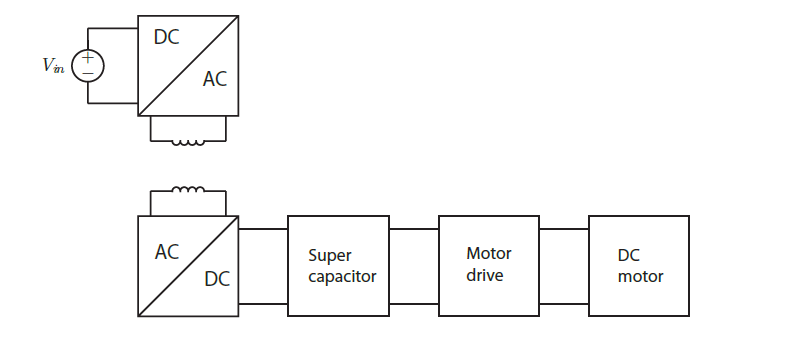
\includegraphics[width=0.8\linewidth]{resource/contactless_charging.png}
	\end{center}
	\caption{The wireless charging system with supercapacitors}
	\label{fig:contactless_charging}
\end{figure}

\section{Power electronics}
The first step in designing our DC/DC converter meant we had to incorporate the used UC3525 Regulating
Pulse Width Modulator and the IRS2001PBF Gate Drivers into a full bridge converter (the
DC/AC step), while at the same time integrating the given overcurrent protection circuit in the correct
way. Since connection schemes for both the UC3525 and the IRS2001PBF were given in their respective
datasheets \cite{uc3525a-datasheet}, \cite{irs2001pbf-datasheet} this did not pose much of a problem. The focus
was not on calculating the resistors and capacitors values, therefore we will not discuss the choices we
made regarding these values. However, we will discuss our choice of the used MOSFET transistors and
diodes. The most important factors in picking the correct transistor for our application were static and
dynamic power dissipation. \\

While choosing a MOSFET	there where three MOSFETs (IPP50CN10N, IPP028N08N3G, PSMN017) available. Our circuit parameters were well within their given margins. This meant that all of them could be used for making a working DC/DC converter. The factor on which the suitability of each MOSFETs was tested is, as already mentioned, the power dissipation. The total dissipation of the MOSFETs can be calculated with

\begin{equation}
P = I_{DS}R_{DS(on)}D +	(C_{in}V_{GS}^2 + C_{out}V_{DS}^2)f_{s}.
\end{equation}

Herein $I_{DS}$ is the drain-source current through the transistor, $R_{DS(on)}$ is the transistors drain-source resistance when switched on, $D$ is the duty-cycle of the PWM control signal, $C_{in}$ and $C_{out}$ are the transistor’s in- and output capacitances, $V_{GS}$ is the gate-source voltage on the
transitor (15 V), $V_{DS}$ is the drain-source voltage on the transistor (15 V) and $f_{s}$ is the switching frequency (100 kHz).  The results of calculating the power dissipation of each transistor are shown in Table~\ref{tab:ass2-powerloss}. 

\begin{table}[H]
	\centering
	\begin{tabular}{c c c c c c c}
		\hline\hline
		MOSFET & $R_{DS(on)}$ & $C_{in}$ & $C_{out}$ & Static loss & Dynamic loss & Total loss \\
		\hline
		IPP50CN10N & \SI{49}{m\ohm} & \SI{822}{pF} & \SI{120}{pF} & \SI{0.098}{W} & \SI{0.021}{W} & \SI{0.119}{W} \\
		IPP028N08N3G & \SI{2.8}{m\ohm} & \SI{10700}{pF} & \SI{2890}{pF} & \SI{0.006}{W} & \SI{0.306}{W} & \SI{0.311}{W} \\
		PSMN017 & \SI{13.7}{m\ohm} & \SI{1573}{pF} & \SI{154}{pF} & \SI{0.027}{W} & \SI{0.039}{W} & \SI{0.066}{W} \\
		\hline
		\end{tabular}
		\caption{MOSFET power loss calculations}
	    \label{tab:ass2-powerloss}
\end{table}

It can be seen in the table that PSMN017 has the lowest power dissipation and thus making it the most suitable MOSFET. As for the diodes we had two different types (SB540, SF61) at our disposal. For choosing a propper diode the power dissipation for each component was calculated once again. When assuming that the output voltage is near constant, the static dissipation, in context of the inverter, is given by
\begin{equation}
	P_s = I V_{fw} D_{d}
\end{equation}
in which $I$ represents the current flowing through the diodes, $V_{fw}$ the forward voltage drop and $D_{d}$ the \textit{diode duty cycle}. The diode duty cycle determines the percentage of time in which current flows through the diode with respect to the switching frequency. $D_{d}$ is given by
\begin{equation}
	D_d = \frac{1}{2}+\arcsin{ \left( \frac{V_{min}}{V_{max}}-1 \right) }
\end{equation}
in which the minumum and maximum output voltage of the inverter is represented by $V_{min}$ and $V_{max}$.

From the calculations it turned out that the SB540 diode dissipated just 56\% of the power dissipated by the SF61 diode. Making SB540 thereby the most appropriate diode for our system. Implementing the PWM-generator, two gate drivers, the overcurrent protection circuit and the rectifier
with overvoltage buzzer circuit resulted in the schematics found in Appendix~\ref{app:schematics}.

\section{Transformer}
As can be seen in Figure~\ref{fig:contactless_charging} the only thing left to complete the DC/DC converter is the air-core transformer. Firstly one must design and build the coils for our transformer. After completing this a compensation circuit can be added. This compensation circuit nullifies the effect of the inductances. The only limiting factor which then remains, is the mutual inductance. Therefore, by moving the coils further apart, the power transfer increases. However, at a certain point the leakage inductances become significant and consequently the power transfer decreases.

Target parameters for the coils were an inner diameter of \SI{50}{cm} for both coils and inductances of \SI{22}{μH} for the secondary coil and \SI{100}{μH} for the primary coil. The actual coils built had the parameters shown in Figure~\ref{tab:ass2-coil-params-meas}.

\begin{table}[H]
	\centering
	\caption{Measured coil parameters}
	\label{tab:ass2-coil-params-meas}
	\begin{tabular}{c c c}
		\hline\hline
		Coil & Inductance & DC-resistance \\
		\hline
		Primary & \SI{94.5}{\micro H} & \SI{250}{m\ohm} \\
		Secondary & \SI{25.2}{\micro H} & \SI{65}{m\ohm} \\
		\hline
		\end{tabular}
\end{table}

Then, we calculated the coils’ mutual inductance and coupling factor via the ostrich approach as given
in \cite{epo4-manual}. The results are shown in Figure~\ref{tab:ass2_coil_mutual}.

\begin{table}[H]
	\centering
	\begin{tabular}{c c c c c}
		\hline\hline
		Distance & Aiding inductance & Opposing inductance & Mutual inductance & Coupling factor \\
		\hline
		\SI{0}{cm} & \SI{184.3}{\micro H} & \SI{58.6}{\micro H} & \SI{314.2}{\micro H} & 0.64 \\
		\SI{2}{cm} & \SI{151.5}{\micro H} & \SI{86.8}{\micro H} & \SI{161.8}{\micro H} & 0.33 \\
		\SI{4}{cm} & \SI{135.6}{\micro H} & \SI{100.0}{\micro H} & \SI{88.9}{\micro H} & 0.18 \\
		\SI{6}{cm} & \SI{127.5}{\micro H} & \SI{107.0}{\micro H} & \SI{51.2}{\micro H} & 0.11 \\
		\hline
		\end{tabular}
		\caption{Mutual inductance and coupling factor at varying distance}
		\label{tab:ass2_coil_mutual}
\end{table}

\section{Testing}
After soldering the
PCB we got from our consultant we hooked it up to an oscilloscope, on which we then measured tidy
square waves for the gate drivers and power outputs, whose frequency and duty-cycle could be varied by
changing the values of the two potmeters in the design. While inspecting the rectifier output waveform,
we obtained a nice DC-signal, with very little ripple, due to the high switching frequency (i.e. compared
to for example the rectifier used during EPO1 at \SI{50}{Hz}). The charging system is also equiped with a compensation circuit as shown in Figure~\ref{fig:ass2_eq_circ}. While designing this we first determined the transfer function.

\begin{equation} \label{eq:ass3-transfer-function}
	|H(s)| = \frac{s M Z_L}{(s M)^2 - (s L_2 + R_2 + (s C_2)^{-1} + Z_L) ( s L_1 + R1 + (s C_1)^{-1}))} .
\end{equation}

With this formula it was possible to simulate the power transfer for a circuit with and without a compensation circuit. The results are available in Figure~\ref{fig:ass2-transfer-function}.

\begin{figure}[H]
	\begin{center}
		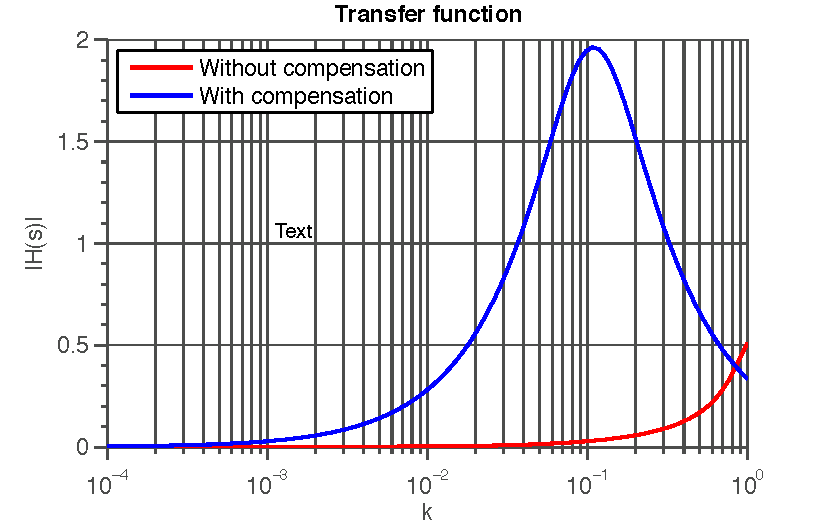
\includegraphics[width=0.8\linewidth]{resource/transfer-function-rc.pdf}
	\end{center}
	\caption{Transfer function with and without compensation}
	\label{fig:ass2-transfer-function}
\end{figure}

\begin{figure}[H]
	\begin{center}
		\begin{subfigure}[h]{0.48\textwidth}
			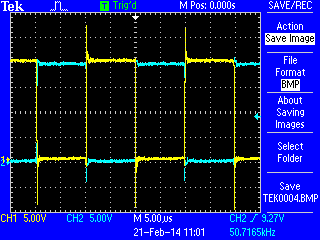
\includegraphics[width=\textwidth]{resource/osc-coil-primary.png}
			\caption{Voltage of the two ends of the primary coil with respect to ground}
			\label{fig:charging-osc-coil-primary}
		\end{subfigure}
		\quad
		\begin{subfigure}[h]{0.48\textwidth}
			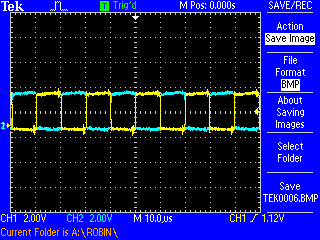
\includegraphics[width=\textwidth]{resource/osc-coil-secondary.png}
			\caption{Voltage of the two ends of the secondary coil with respect to ground}
			\label{fig:charging-osc-coil-secondary}
		\end{subfigure}
	\end{center}
	\caption{Inverter voltage waveforms at primary and secondary side}
\end{figure}

To test our design, we studied its waveforms using the oscilloscope. Screenshots of this are shown in Figure~\ref{fig:charging-osc-coil-primary} and Figure~\ref{fig:charging-osc-coil-secondary}. From these waveforms may be concluded that the inverter generates a correct waveform and this waveform is transferred correctly by the two coils. We measured a steady DC-signal at the load. The results are displayed in Table~\ref{tab:ass2_power}.

\begin{table}[H]
	\centering
	\begin{tabular}{c c c c c c c}
		\hline\hline
		Distance & Source voltage & Source current & Source power & Load voltage & Load power & Efficiency \\
		\hline
		\SI{2}{cm} & \SI{19.998}{V} & \SI{1.2472}{A} & \SI{24.942}{W} & \SI{14.8}{V} & \SI{21.3}{W} & \SI{85.6}{\percent} \\
		\hline
		\end{tabular}
			\caption{Power transfer measurements - compensated}
			\label{tab:ass2_power}
\end{table}

\begin{figure}[H]
	\begin{center}
		% 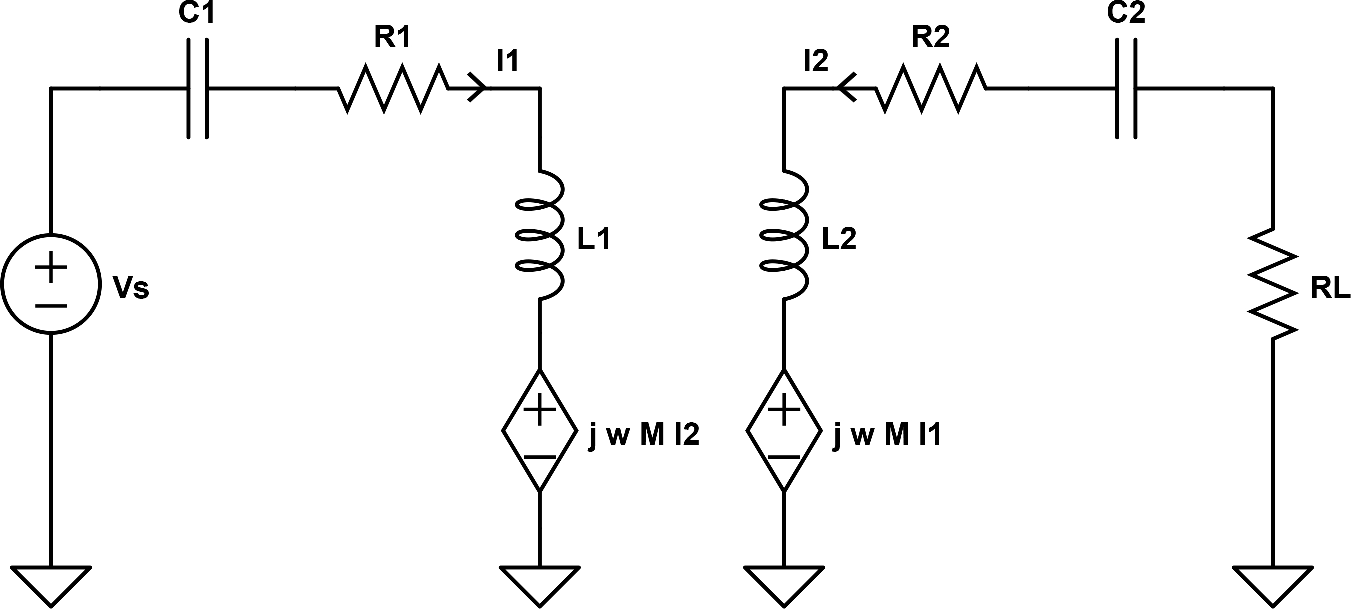
\includegraphics[width=0.8\linewidth]{resource/cpt-equivalent-circuit-rc.pdf}
		\begin{circuitikz}[scale=1.2]
			 \draw (0,0) node[ground] {} to[american voltage source,l=$V_s$] (0,4)
				to[C, l=$C_1$] (2,4)
				to[R, l=$R_1$] (4,4)
				to[L, l=$L_1$] (4,2);

			\draw (4,0) node[ground] {} to[american controlled voltage source, l=$j \omega M I_2$, i<=$I_1$] (4,2);

			\draw (6,0) node[ground] {} to[american controlled voltage source, l_=$j \omega M I_1$, i<=$I_2$] (6,2)
				to[L, l=$L_2$] (6,4)
				to[R, l=$R_2$] (8,4)
				to[C, l=$C_2$] (10,4)
				to[R, l=$R_L$] (10,0) node[ground] {};
		\end{circuitikz}
	\end{center}
	\caption{Equivalent circuit with compensation}
	\label{fig:ass2_eq_circ}
\end{figure}

\section{Demonstration}
The charging system's functionality had to be demonstrated at a distance of \SI{6}{cm}. Therefore the performance of the system had to be optimized for a distance at \SI{6}{cm}. Requirements were that the system was fully charged to \SI{20}{V} within four minutes, the system had to be in solid resonance and the charging limiter should be working. Since the system had to be in solid resonance the frequency was no option of variation to maximize charging speed. For this reason the duty cycle was changed in order to maximize the charging speed of the system at \SI{6}{cm}. This was done by trial and error. The result was a system at resonance for a frequency at \SI{100}{kHz}, a duty cycle of 40\% and a maximal charging speed of 3:45 minutes. Our charging system met all the requirements. 
\end{document}


